\subsection{Clustering Losses}

\begin{frame}
	\frametitle{Clustering Losses}
	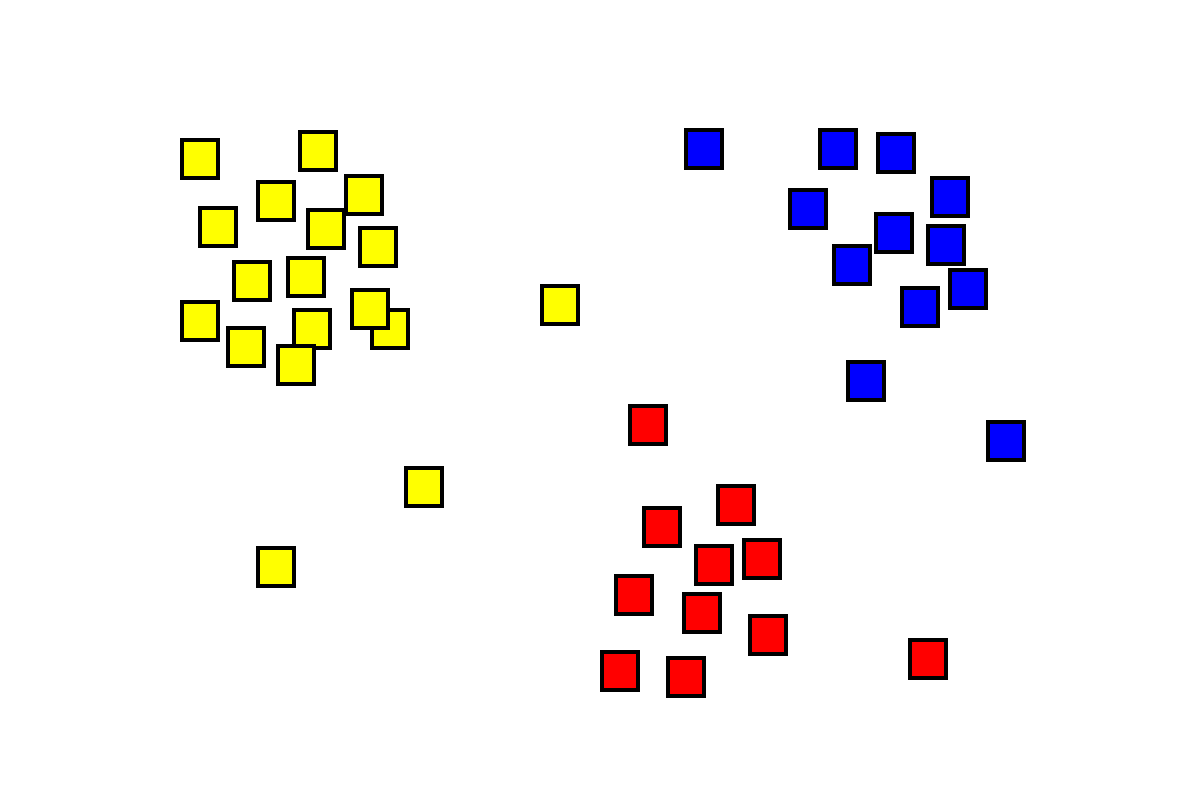
\includegraphics[scale=0.2, center]{images/clust1}
\end{frame}

\begin{frame}
	\frametitle{Mean Entropy Loss}
	\begin{itemize}
		\item The mean entropy loss over a batch of size $T$ is gives by:
			\begin{block}{Mean Entropy Loss}
				\begin{equation*}
					J_M = \frac{1}{T}\sum_{t=1}^{T}H(\mathbf{q}_t)
				\end{equation*}
				where $H$ is the entropy and $\mathbf{q}_t = f(\mathbf{X}_t; \Theta)$ is the output
				probability distribution for image $\mathbf{X}_t$
			\end{block}
		\item This increases the confidence of the predicted class
	\end{itemize}
\end{frame}

\begin{frame}
	\frametitle{Negative Batch Entropy Loss}
	\begin{itemize}
		\item The spread of outputs should be similar to the spread of dataset
			label distribution
			\begin{block}{Negative Batch Entropy Loss}
				\begin{equation*}
					\label{eq:nbel}
					J_B = D_{KL} (\frac{1}{T}\sum_{t=1}^{T}\mathbf{q}_t \lVert \mathbf{d})
				\end{equation*}
				where $D_{KL}$ is the KL-divergence, $\mathbf{q}_t = f(\mathbf{X}_t; \Theta)$ is
				the output probability distribution for image $\mathbf{X}_t$, and $\mathbf{d}$ is
				the label probability distribution in $\mathcal{S}$
			\end{block}
	\end{itemize}
\end{frame}

\begin{frame}
	\frametitle{Negative Batch Entropy Loss}
	\begin{itemize}
		\item In case of datasets with uniform distribution of classes
			\begin{block}{NBEL for Uniform Dataset Label Distribution}
				\begin{equation*}
					J_B = -H(\frac{1}{T}\sum_{t=1}^{T}\mathbf{q}_t)
				\end{equation*}
			\end{block}
		\item This is the case for ImageNet and CIFAR-10
	\end{itemize}
\end{frame}

